\chapter{TravelatAR : 地表面近似テクスチャーのアニメーション重畳表示による歩行速度制御システム}
本システムではユーザの視界に映る床へ現実の床を模したバーチャル床が被験者に対して前から流足元へ流れてくるようなアニメーション重畳表示する.
これにより,被験者の自己運動感覚を操作し意味解釈を必要としない歩行速度操作を行う.
\section{システム概要}
\figref{fig:gaiyo}に本システムの概要を示す.
本システムでは被験者にARグラスを装着してもらう.
これにより,仮想空間に存在する現実の床を模したバーチャル床をユーザの視界の床へアニメーション重畳表示する.
\begin{figure}[h]
    \centering
    \fbox{
        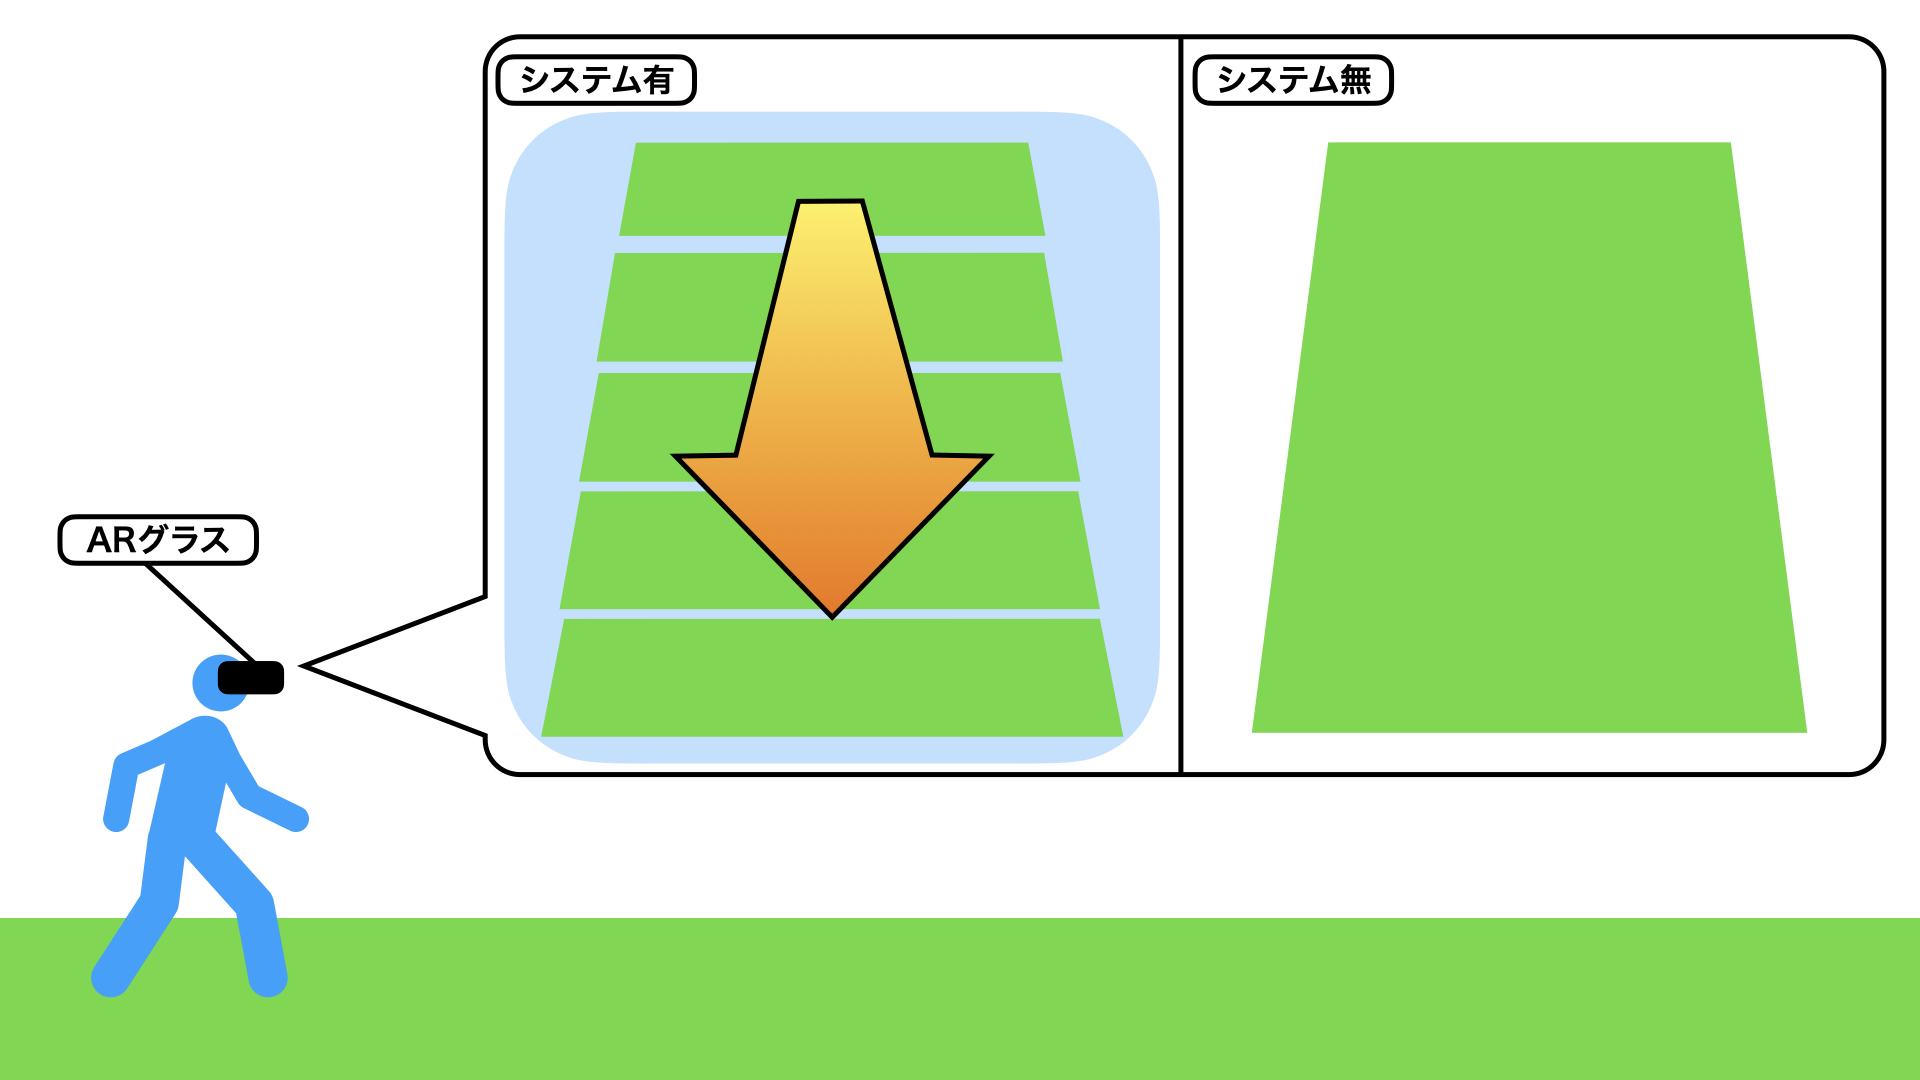
\includegraphics[width=0.8\linewidth]{fig/gaiyo.001.jpeg}
    }
    \caption{システム概要図}
    \label{fig:gaiyo}
\end{figure}

\begin{figure}[ht]
    \centering
    \fbox{
        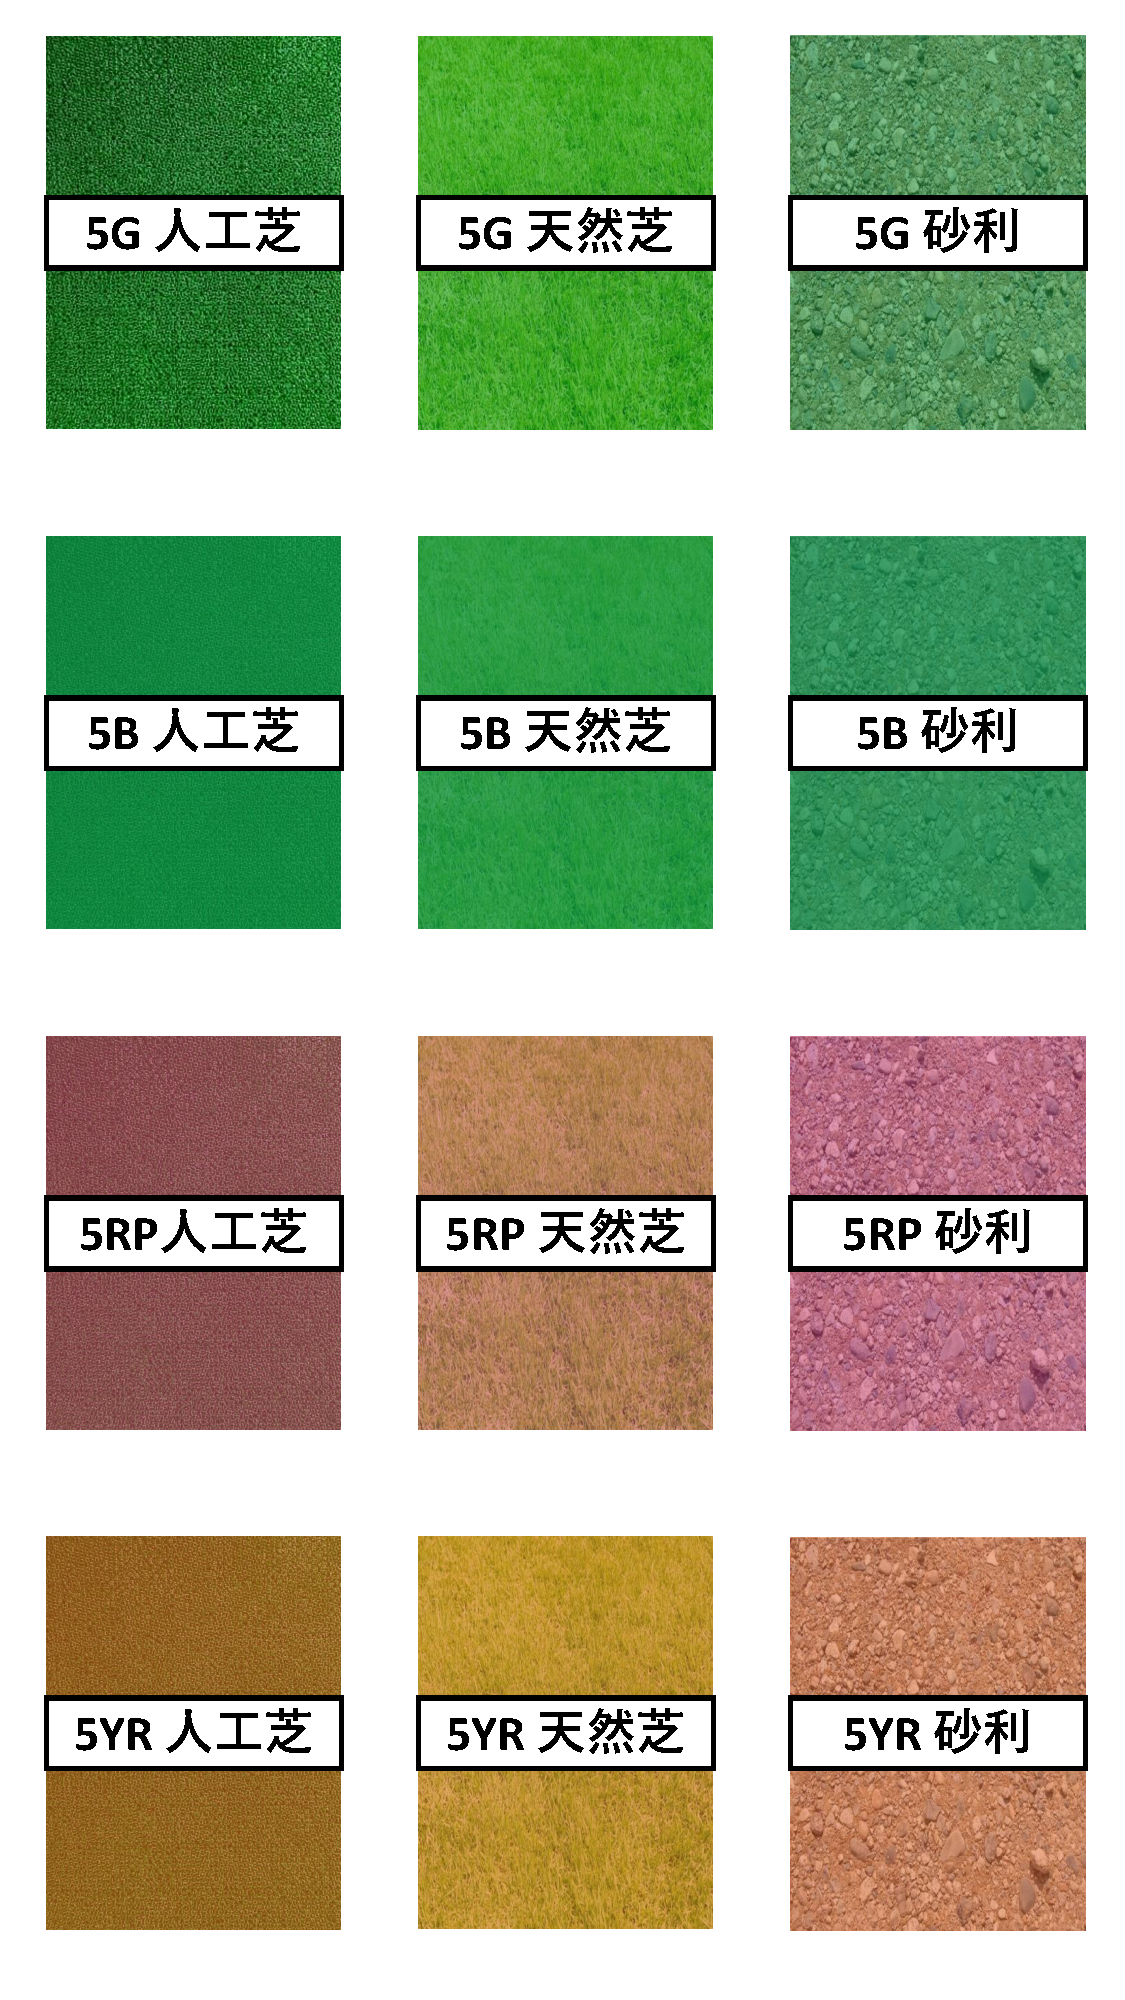
\includegraphics[width=0.7\linewidth]{fig/マテリアル.pdf}
    }
    \caption{リアルテクスチャ(5G人工芝)・Nonリアルテクスチャ一覧}
    \label{fig:Nrial}
\end{figure}


\section{リアルテクスチャ}
ユーザが歩く道の地表面に近似したテクスチャを作成する.
本システムでは,これらのテクスチャをバーチャル床にアタッチし被験者の視界の床へアニメーション重畳表示を行う.
本実験では人工芝の道を歩くことを想定したリアルテクスチャ作成した.
また,リアルテクスチャの比較対象となる地表面に近似していないNonリアルテクスチャを複数作成した.

\section{Nonリアルテクスチャ}
\figref{fig:Nrial}にリアルテクスチャとNonリアルテクスチャの一覧を示す.
リアルテクスチャは,色と模様を地表面に近似させ,作成している.
色は,人工芝と同じ色である5G,色相環で5Gの反対に位置する5RP,それらの中間に位置する5YR,5Bを使用した\cite{color}.
模様は,人工芝に近似させたもの,人工芝に近いものとして天然芝,そして,人工芝に近似させない物として砂利を用意した.
今回Nonリアルテクスチャはリアルテクスチャを含む12通りで作成した.


\section{バーチャル床}
バーチャル床は仮想空間内に存在する仮想オブジェクトである.
このオブジェクトに上記で説明したリアルテクスチャかNonリアルテクスチャをアタッチし
ARグラスを通してユーザへ次々と提示する.
また,このオブジェクトはシステムの負荷を下げるため,ユーザが踏んだ際に消える設定となっている.
ユーザへ提示される際,ユーザの視界の床に前から迫ってくるなどのアニメーション重畳表示される.

\section{実装}
本システムはunityを用いて作成を行った\cite{unity}.
今回の実験では歩く道が固定であったため,バーチャル床を発生させる位置をユーザの正面20m先に固定した.
発生するバーチャル床はユーザの頭の位置から1.6m下の位置を移動する.この1.6mは被験者たちの身長から調整を行った.